En este capítulo se detalla cada uno de los puntos llevados a cabo para la realización de este proyecto, empezando por definir la propuesta realizada, luego explicar el proceso ingenieril llevado a cabo y terminar desglosando el trazado de la ejecución de este proyecto.

\section{Propuesta}

El trabajo propuesto tiene como objetivo la creación de un elemento software funcional que, usando el paradigma lógico explicado en la Sección \ref{asp}, permita la generación de un escenario jugable que pueda ser ejecutado en el juego Freeciv, como se indica en la Sección \ref{subsec:freeciv}. Así mismo incluirá una interfaz gráfica interactuable que permitan al usuario marcar que zonas del terreno deben generarse y cuales no, indicando su contenido antes de lanzar el proceso de generación.

\subsection{Formato del escenario de Freeciv}

Como uno de los puntos fuerte de este trabajo tiene que ver con la generación de escenarios, este sistema tiene que tener como salida un mapa válido que sea leído correctamente por el juego Freeciv. Es por eso que explicaré en detalle el formato usado. \\

Para empezar, el formato se basa en archivo de texto plano que contiene varios campos, haciendo que sea lo más simple posible y que en la teoría se pueda modificar a mano.

\begin{lstlisting}[caption=Ejemplo de formato de mapa,label=lst:format]
[scenario]
is_scenario=TRUE
name=_("My map")
description=_("This map is a example.")
players=TRUE

[savefile]
options=" +version2"
version=20
reason="Scenario"
rulesetdir="classic"
[...]

[settings]
set={"name","value","gamestart"
          "generator","SCENARIO","RANDOM"
          "mapsize","FULLSIZE","FULLSIZE"
          "maxplayers",::PLAYERS::,::PLAYERS::
          "topology","","WRAPX|ISO"
          "xsize",50,12
          "ysize",50,12
          [...]
}
set_count=9

[map]
have_huts=FALSE
t0000="h+hf  aaaa    ff"
t0001="dgg    aat    ff"
t0002="hhh           pp"
t0003="hmp        ggghh"
t0004="hmh       s dghf"
t0005=" dg      phffpm "
t0006="                "
t0007="aa     sdg    aa"
t0008="aa      h     aa"
t0009="       jff p    "
t0010="mh      s pdp pm"
t0011="gf       pdhh   "
t0012="        gpsg   p"
t0013="      h  hh     "
t0014="hff         gg s"
t0015="m+h   aaaa   m f"
startpos_count=5
startpos={"x","y","exclude","nations"
          0,2,FALSE,"Russian"
          9,11,FALSE,"Spanish"
          14,0,FALSE,""
          2,5,FALSE,""
          12,3,FALSE,""
}
b00_0000="0000000000000000"
[...]
r00_0000="0000000000000000"
[...]
\end{lstlisting}

Como se puede comprobar en el Listado \ref{lst:format}, el archivo que contiene un mapa se divide en varias secciones de datos, los cuales se marcan con un título entre corchetes. De los definidos por Freeciv, se puede destacar algunos.

\begin{itemize}
	\item \texttt{scenario}: Configura los ajustes básicos del mapa creado, como puede ser el nombre del mismo (con el campo \texttt{name}) o una breve descripción (con el campo \texttt{description}).
	\item \texttt{savefile}: Establece los valores por defecto de las opciones de juego, como puede ser la versión de Freeciv mínima (con el campo \texttt{options}), el conjunto de reglas de juego (con el campo \texttt{rulesetdir}) o las tecnologías disponibles (se establece en la lista guardada por \texttt{technology\_vector} y se indica el número de elementos en \texttt{technology\_size}).
	\item \texttt{settings}: Se puede definir una lista de valores del mapa y la topología del mismo (que se explica en detalle en la Sección \ref{subsubsec:topology}) en el campo \texttt{set}. El número de valores definidos se guarda en el campo \texttt{set\_count}.
	\item \text{map}: En esta sección se indica cada uno de los valores de terreno de la rejilla del mapa (en los campos \texttt{t00\_XXXX}), así como la lista de puntos de inicio de jugadores (definidos en la lista \texttt{startpos} e indicado el tamaño de la lista en \texttt{startpos\_count}), las capas con recursos o incluso las capas de ríos.
\end{itemize}

\subsubsection{Topología del mapa}
\label{subsubsec:topology}

El mapa es siempre una rejilla de dos dimensiones en el que cada celda es una baldosa o \textit{tile}. Esta rejilla puede estar configurada de varias maneras con la variable \texttt{topology} en la sección \texttt{settings}.

\begin{itemize}
	\item \texttt{warpx}: La topología de escenario es como un mapa terrestre, es decir el eje Este-Oeste se junta.
	\item \texttt{warpy}: La topología del escenario junta el eje Norte-Sur.
	\item \texttt{warpx warpy}: La topología del escenario es un toroide, es decir, tiene forma de donuts.
	\item \texttt{iso}: La rejilla del escenario es isométrico.
	\item \texttt{hex}: La rejilla del escenario es hexagonal.
	\item \texttt{iso hex}: La rejilla del escenario es en forma de panel de abeja.
\end{itemize}

\subsubsection{Terrenos disponibles por defecto}
\label{subsubsec:terrain}

En Freeciv, cada celda de la rejilla del mapa contiene una baldosa de terreno único, que viene definido por un identificador único, el cual puede ser uno de los siguientes:

\def\arraystretch{1.5}%  1 is the default, change whatever you need

\begin{table}[!h]
	\begin{tabular}{ p{0.7\textwidth} c c }
		\bfseries{Descripción} & \bfseries{ID} & \bfseries{Imagen} \\
		\hline
		\textit{Pradera}: Es uno de los terrenos más comunes. Las unidades se pueden mover fácilmente. & \texttt{g} & \adjustimage{height=2em,valign=t}{images/grassland.png} \\
		\textit{Llanura}: Es otro terreno muy común. Se puede usar para crear carreteras. & \texttt{p} & \adjustimage{height=2em,valign=t}{images/plains.png} \\
		\textit{Colinas}: Las unidades se mueven lentamente. Es uno de los terrenos con mayor bonus defensivo (200\%). & \texttt{h} & \adjustimage{height=2em,valign=t}{images/hills.png} \\
		\textit{Bosque}: Produce una unidad de producción (madera) con la que construir edificaciones. Tiene un bonus defensivo de 150\% & \texttt{f} & \adjustimage{height=2em,valign=t}{images/forest.png} \\
		\textit{Jungla}: Puede llegar a producir 4 unidades de producción si se encuentran con recursos de gemas o fruta. & \texttt{j} & \adjustimage{height=2em,valign=t}{images/jungle.png} \\
		\textit{Montanas}: Es el terreno con mayor bonus defensivo (300\%). Solo las unidades aéreas (aviones, cazas, etc) pueden atravesarla. & \texttt{m} & \adjustimage{height=2em,valign=t}{images/mountains.png} \\
		\textit{Desierto}: Normalmente solo se puede usar para crear carreteras, pero si hay un modificador de oasis puede generar hasta 3 unidades de producción. & \texttt{d} & \adjustimage{height=2em,valign=t}{images/desert.png} \\
		\textit{Pantano}: Se puede irrigar rápidamente. Puede producir de 5 a 9 unidades de producción si se encuentra con recursos como tundra o con especias. & \texttt{s} & \adjustimage{height=2em,valign=t}{images/swamp.png} \\
		\textit{Tundra}: Solo se pueden crear carreteras. & \texttt{t} & \adjustimage{height=2em,valign=t}{images/tundra.png} \\
		\textit{Glacier}: Ninguna de las unidades puede cruzarlo. & \texttt{a} & \adjustimage{height=2em,valign=t}{images/glacier.png} \\
	\end{tabular}
	\caption{Tipos de terreno}\label{table:terrains1}
\end{table}

\begin{table}[!h]
	\begin{tabular}{ p{0.7\textwidth} c c }
		\bfseries{Descripción} & \bfseries{ID} & \bfseries{Imagen} \\
		\hline
		\textit{Mar}: Todas las unidades acuáticas pueden cruzarlo. Puede producir 2 unidades de producción si se encuentra con un banco de peces & & \adjustimage{height=2em,valign=t}{images/sea.png} \\
		\textit{Océano}: Solo las grandes embarcaciones y submarinos pueden pasar por encima. & \texttt{:} & \adjustimage{height=2em,valign=t}{images/ocean.png} \\
	\end{tabular}
	\caption{Tipos de terreno}\label{table:terrains2}
\end{table}

\section{Proceso de ingeniería}

\subsection{Metodología}

\subsection{Gestión del proyecto}

\section{Análisis del software}

Una vez definido el sistema y planificada su construcción, se ha realizado un análisis en donde se identifican los requisitos que debe cumplir el software una vez terminado el proyecto.

\subsection{Requisitos funcionales}
\label{subsec:funcrequirements}

Los requisitos funcionales son aquellas condiciones indispensables que estipulan las funcionalidades que debe proporcional el sistema. Para este proyecto se ha recogido los diferentes requisitos:

\begin{itemize}
	\item Generación de un mapa que sea legible por el videojuego Freeciv.
	\item Permitir añadir restricciones sobre ciertas zonas del mapa.
	\item Poder guardar y recuperar el mapa en un formato sencillo.
\end{itemize}

\subsection{Requisitos no funcionales}

Los requisitos no funcionales, por su contra, son aquellas condiciones indispensables que debe cumplir el sistema a la hora de diseñar e implementar. Para este proyecto se han tenido en cuenta estos requisitos:

\begin{itemize}
	\item Eficiencia y eficacia: El generador debe responder en el menor tiempo posible arrojando una respuesta óptima.
	\item Escalabilidad: El generador debe trabajar con mapas de diferentes tamaños, por lo que el sistema debe poder soportar cualquier tamaño de entrada.
	\item Usabilidad: La interfaz gráfica debe ser lo más sencilla posible, evitando que el usuario tenga que realizar tareas tediosas a la hora de construir mapas.
\end{itemize}

\section{Diseño del sistema}

Una vez definidos los requisitos se ha procedido a realizar el diseño software del sistema en cuestión, empezando a concretar la arquitectura propuesta y luego desarrollando los casos de uso y diagramas de clases.

\subsection{Arquitectura software}
\label{subsec:arquitectura}

Debido a que el sistema cuenta con una interfaz gráfica y un módulo que se encargará de generar el mapa, el sistema estará dividido en dos partes concretas tal y como se puede ver en la Figura \ref{fig:arquitectura}:

\begin{itemize}
	\item Una parte que será la aplicación gráfica, que actuará en todo momento como \textit{Front-end} de cara al usuario. Esta parte sigue la estructura Modelo-Vista-Controlador (MVC), en donde el controlador se encargará de hacer de puente entre la interfaz gráfica, que es lo que manipulará el usuario, y los datos guardados en memoria. Así mismo proporcionará las funcionalidades básicas del sistema como guardar o cargar el mapa y crear un mapa en blanco.
	\item La segunda parte actuará como \textit{Back-end}, que se encargará de generar el mapa mediante un programa lógico escrito en ASP que se ejecutará Clingo. Contiene un controlador que se encargará de hacer la llamada a Clingo y de obtener su resultado, y luego otro controlador que se encargará de llamar primeramente al programa lógico que genere las regiones y luego, dada una región, rellene las casillas de la región. Para ello primeramente define que zonas son tierra y que zonas son agua, y con las zonas con tierra se rellenan con cordilleras y con áreas bióticas (las cuales son zonas grandes que contienen un solo tipo de terreno). Una vez realizado terminará generando los mares y los puntos de inicio para los jugadores.
\end{itemize}

\begin{figure}[!h]
	\centering
	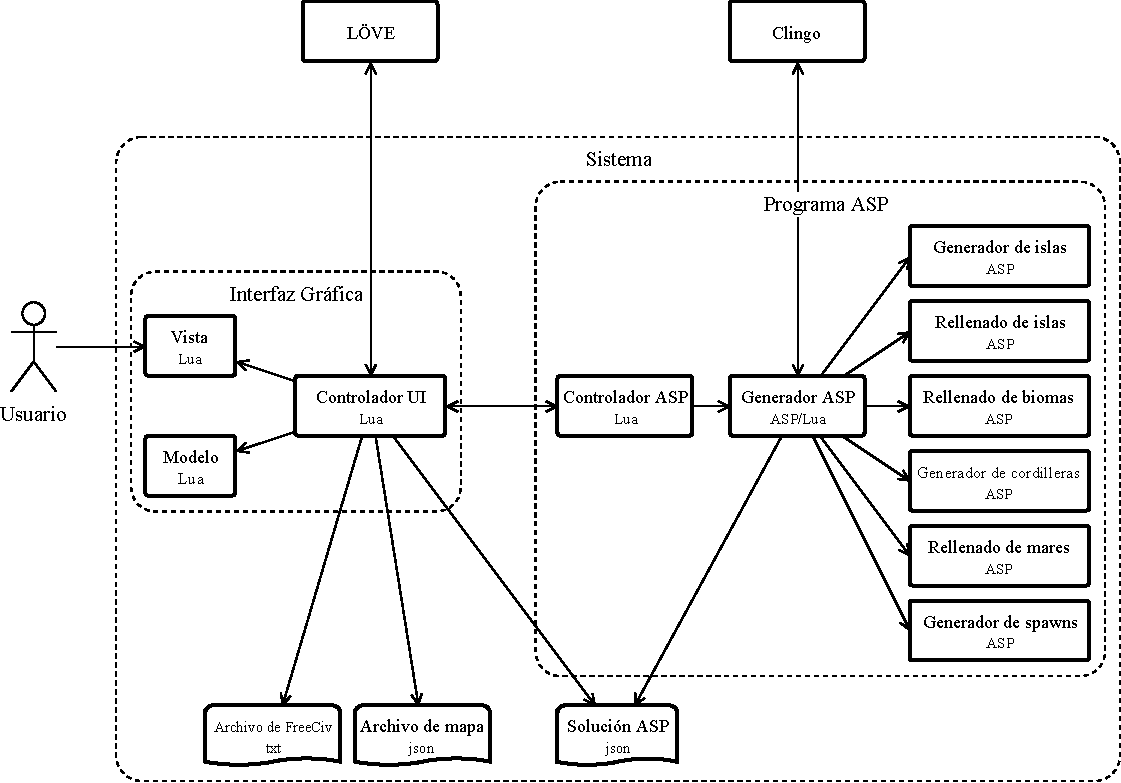
\includegraphics[width=\textwidth]{images/arquitectura.pdf}
	\caption{Arquitectura del sistema}
	\label{fig:arquitectura}
\end{figure}

Tanto el controlador de la interfaz de usuario como el controlador del programa ASP se ejecutarán en paralelo, pudiendo enviarse información de un controlador a otro para saber cuando hay que empezar una generación o si esta terminó. A pesar de esto, los resultados de la generación de ASP se guadarán en un archivo intermedio para evitar enviar gran cantidad de datos entre los elementos.

\subsection{Casos de uso}
\label{subsec:cases}

El sistema tiene en cuenta que se usará en todo momento por un único usuario, el cual llevará a cabo todas las funcionalidades propuestas en la Sección \ref{subsec:funcrequirements} a través de una interfaz gráfica que se explica en la Sección \ref{subsec:mockups}. Estos requisitos funcionales se transforman, por tanto, en los casos de uso del sistema que se proponen el la Figura \ref{fig:cases}.

\begin{figure}[!h]
	\centering
	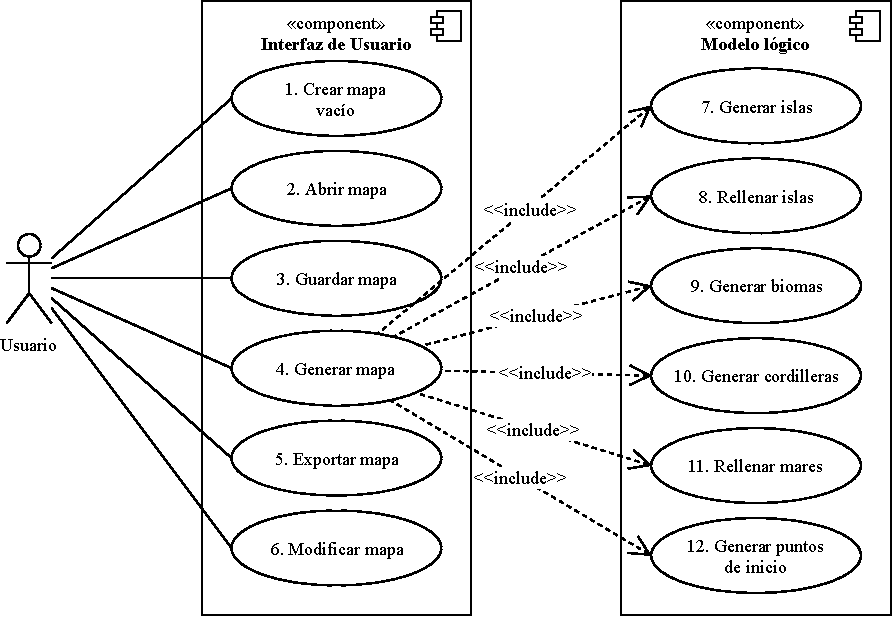
\includegraphics[width=\textwidth]{images/casos-de-uso.pdf}
	\caption{Casos de uso del sistema propuesto}
	\label{fig:cases}
\end{figure}

\subsection{Pantallas del sistema}
\label{subsec:mockups}

El proyecto propuesto está pensado para ser usado a través de una interfaz gráfica de usuario, la cual es modelada mediante un patrón MVC como se indica en la Sección \ref{subsec:arquitectura}. Esta interfaz está dividida en varias vistas, las cuales corresponden con los casos de uso propuestos contra los que el usuario interacciona directamente en la Sección \ref{subsec:cases}.

\begin{itemize}	
	\begin{figure}[!h]
		\centering
		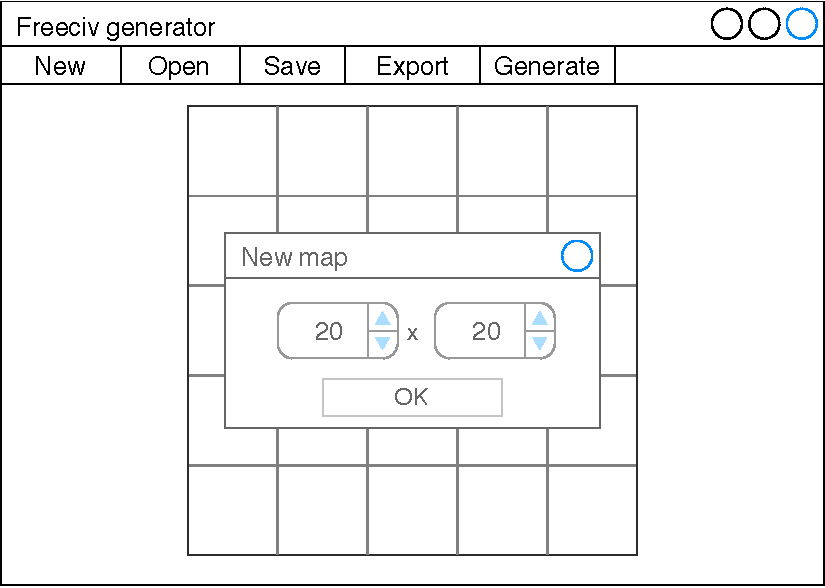
\includegraphics[width=0.5\textwidth]{images/new-map.pdf}
		\caption{Pantalla de nuevo mapa}
		\label{fig:newmock}
	\end{figure}
	
	\item 1. Crear mapa vacío: Se acciona cuando el usuario presiona en el botón de ``Crear mapa'' en la barra de herramientas, lo que despliega una ventana emergente parecida a la Figura \ref{fig:newmock}. Aquí el usuario puede indicar el tamaño del mapa a crear y pulsar el botón de ``Aceptar''. Con esto el sistema muestra una rejilla vacía.

	\begin{figure}[!h]
		\centering
		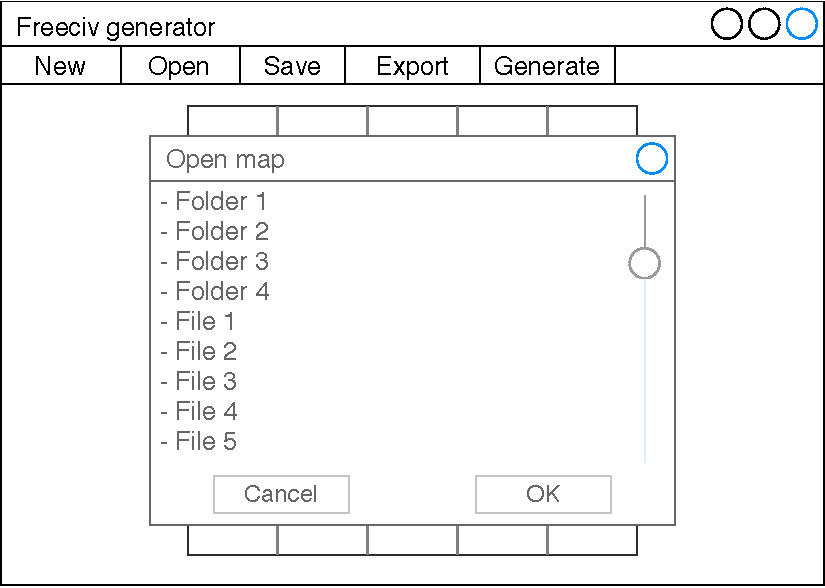
\includegraphics[width=0.5\textwidth]{images/open-map.pdf}
		\caption{Pantalla de abrir archivo de mapa}
		\label{fig:openmock}
	\end{figure}

	\item 2. Abrir mapa guardado en disco: Se inicia cuando el usuario presiona en el botón de ``Abrir mapa'' en la barra de herramientas, lo que despliega una ventana emergente parecida a la Figura \ref{fig:openmock}. Aquí el usuario navega a través de una lista que representa los archivos guardados en disco y selecciona un archivo anteriormente guardado por la aplicación que representa un mapa. El sistema procede a cargarlo y mostrar los datos del mapa en la rejilla principal.
	
	\begin{figure}[!h]
		\centering
		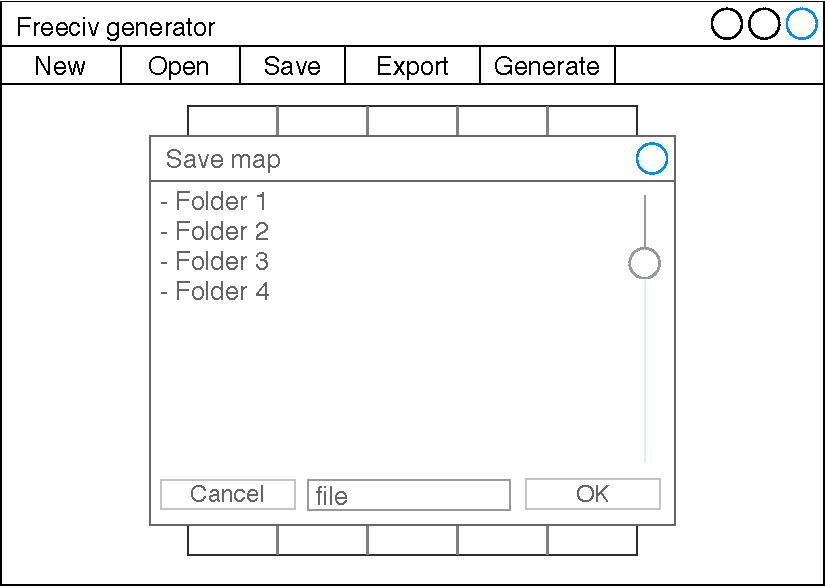
\includegraphics[width=0.5\textwidth]{images/save-map.pdf}
		\caption{Pantalla de guardar mapa}
		\label{fig:savemock}
	\end{figure}
	
	\item 3. Guardar mapa en disco: Se inicia cuando el usuario presiona en el botón de ``Guardar mapa'' en la barra de herramientas, mostrando una ventana emergente como la de la Figura \ref{fig:savemock}. Aquí el usuario navega por las carpetas guardadas en disco a través de una lista y selecciona una donde se guardará. Además, escribe el nombre del nuevo archivo en un campo de texto debajo de esta lista y acepta. El sistema procede a transformar los datos del mapa en un fichero que se guarda en disco donde el usuario indicó.
	
	\begin{figure}[!h]
		\centering
		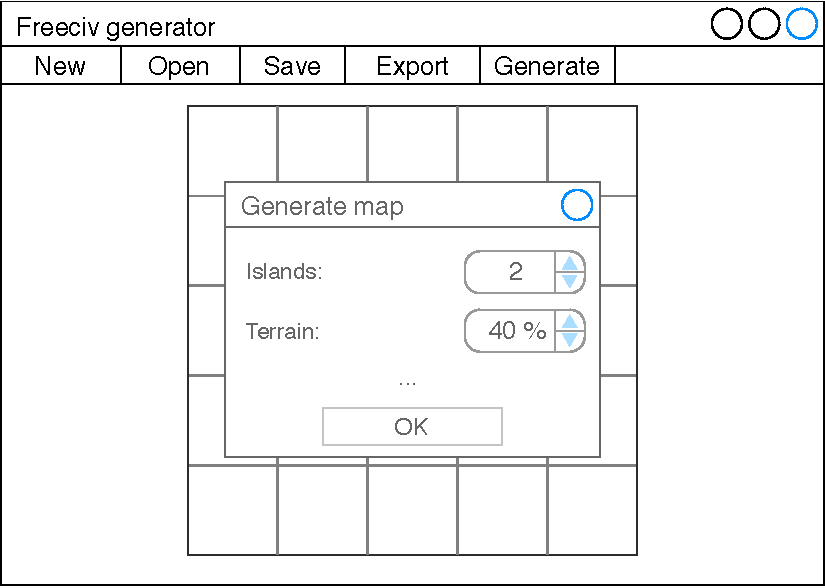
\includegraphics[width=0.5\textwidth]{images/generate-map.pdf}
		\caption{Pantalla de generar mapa}
		\label{fig:generatemock}
	\end{figure}
	
	\item 4. Generar mapa: Se inicia cuando el usuario acciona el botón de ``Generar mapa'' en la barra de herramientas, haciendo que el sistema muestre una ventana emergente parecida a la Figura \ref{fig:generatemock}. Aquí el usuario indica los parámetros que prefiera en la generación y acepta. En sistema procede a llamar a la parte del programa lógico creado en ASP, la cual va ejecutando cada uno de los casos de uso. Entre medias, el sistema lanza una vista como la de la Figura \ref{fig:waitingmock} para proporcionar retro-alimentación al usuario. Una vez acabada la generación, el sistema muestra en la rejilla principal con el mapa que se ha generado finalmente.

	\begin{figure}[!h]
		\centering
		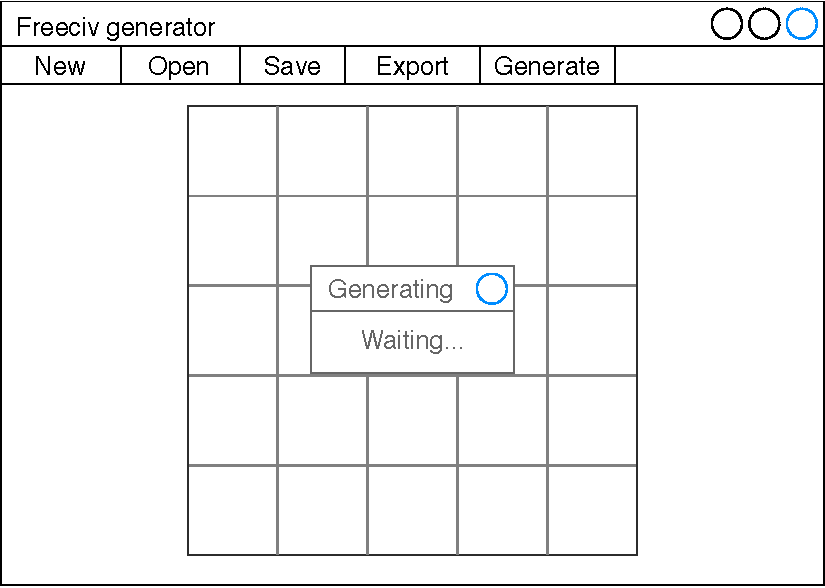
\includegraphics[width=0.5\textwidth]{images/waiting-mock.pdf}
		\caption{Pantalla con el mensaje de espera}
		\label{fig:waitingmock}
	\end{figure}
	
	\item 5. Exportar mapa al formato de Freeciv: Se inicia cuando el usuario presiona en el botón de ``Exportar mapa'' en la barra de herramientas, mostrando una ventana emergente como la de la Figura \ref{fig:exportmock}. Aquí el usuario navega por las carpetas guardadas en disco a través de una lista y selecciona una donde se guardará. Además, escribe el nombre del nuevo archivo en un campo de texto debajo de esta lista y acepta. El sistema procede a transformar los datos del mapa en un fichero reconocible por Freeciv y se guarda en disco donde el usuario indicó.
	
	\begin{figure}[!h]
		\centering
		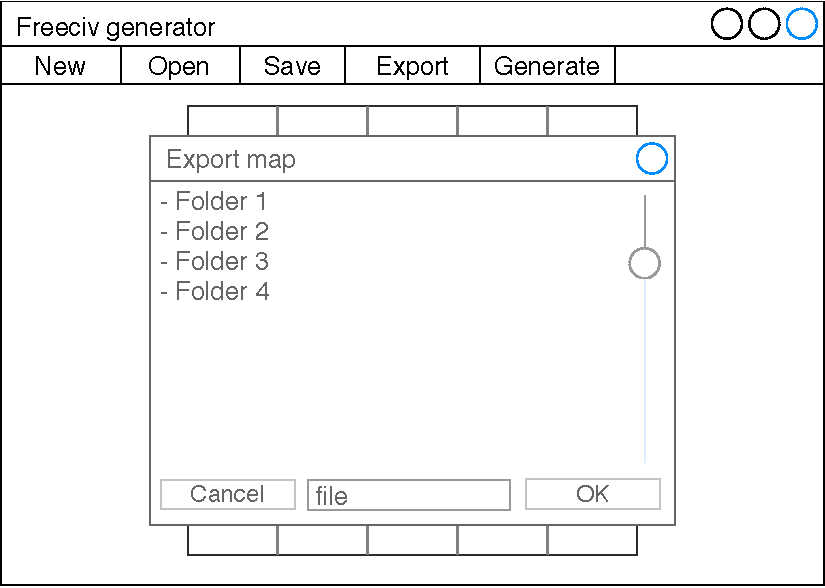
\includegraphics[width=0.5\textwidth]{images/export-map.pdf}
		\caption{Pantalla de exportar mapa}
		\label{fig:exportmock}
	\end{figure}
	
	\item 6. Modificar mapa: Se inicia cuando el usuario presiona sobre una de las celdas de la rejilla como en la Figura \ref{fig:mainmock}. El sistema pasará a cambiar el terreno de la celda por otro, realizando un ciclo en el momento en el que no quede ninguna opción nueva.
	
	\begin{figure}[!h]
		\centering
		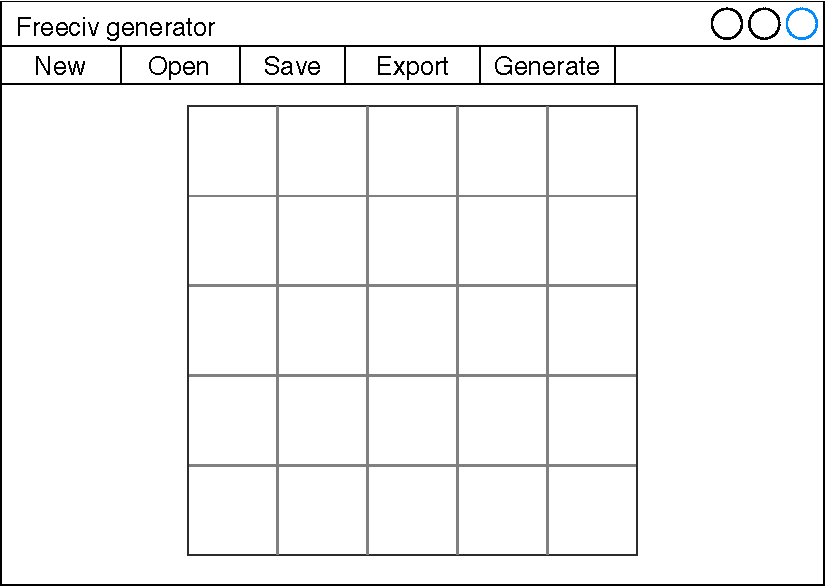
\includegraphics[width=0.5\textwidth]{images/aplicacion.pdf}
		\caption{Pantalla principal de la aplicación}
		\label{fig:mainmock}
	\end{figure}

\end{itemize}

\subsection{Implementación}

Una vez analizado el proyecto en cuestión, pasaré a detallar el diseño de cada uno de los diferentes componentes del sistema en su construcción, indicando mediante diagramas como se integran los diferentes elementos. \\

Como ya se indicó en la Sección \ref{subsec:lua}, el lenguaje de programación Lua no tiene un paradigma de programación orientado a objetos basados en clases, más se ha preferido que en la realización de este sistema se use el módulo \textit{class.lua} de la biblioteca \textit{HUMP}\footnote{https://github.com/vrld/hump} para una organización lo más estructurada posible. Así mismo, también hay que destacar que el lenguaje tampoco soporta la manipulación de archivos en formato JSON, por lo que se ha usado el módulo \textit{json.lua}\footnote{https://github.com/rxi/json.lua}, el cual permite transformar un texto en formato JSON a tipos compatibles en Lua. \\

Por último, indicar que para la realización de las vistas de la interfaz de usuario se ha usado la biblioteca \textit{SUIT}\footnote{https://github.com/vrld/SUIT}, que permite generar una interfaz gráfica en modo inmediato de forma sencilla sobre LÖVE, pudiendo realizar un prototipo de los elementos más rápidamente y con más flexibilidad que con otro tipo de bibliotecas gráficas, como puede ser GTK+\footnote{https://www.gtk.org/}. Por otra parte, habrá elementos gráficos más complejos (como pueden ser diálogos de selección de ficheros o ventanas emergentes) que se tendrán que generar a mano, tal y como se expone en la Sección \ref{subsubsec:widgets}.

\subsubsection{Clase principal}
\label{subsubsec:main}

Como se puede ver en la Figura \ref{fig:mainclass} se ha diseñado la clase principal \texttt{Main}, la cual es una clase estática que sirve de controlador para las vistas y el modelo. Implementa los casos de uso de la interfaz descritos en la Sección \ref{subsec:cases} en los métodos \texttt{\_newMap}, \texttt{\_openMap}, \texttt{\_saveMap}, \texttt{\_exportMap} y \texttt{\_generateMap}, que son eventos que se llaman desde los diálogos emergentes tal y como se explica desde la Sección \ref{subsubsec:widgets}. Para el caso de uso de modificar el mapa, la tarea recae en la clase \texttt{Editor}, que se explica en detalle en la Sección \ref{subsubsec:client}. \\

Con respecto al motor gráfico LÖVE, este usa varias funciones predefinidas cuando se activan distintos eventos, los cuales llaman a los métodos públicos de la clase principal:

\begin{itemize}
	\item El método \texttt{init} es llamado en la función \texttt{love.load} la primera vez que se ejecuta el programa. Sirve para cargar los elementos gráficos e iniciar el resto de clases que serán usadas por el programa.
	\item Como LÖVE es un motor para programación de videojuegos, la función \texttt{love.update} es llamada en un bucle de eventos internos antes de actualizar la pantalla. Esta función llama al método homónimo de la clase principal, el cual prepara las vistas de la interfaz para su pintado en pantalla y llama a los métodos correspondientes según los eventos producidos en las vistas.
	\item Una vez actualizada la lógica, se procede al pintado de pantalla mediante la función \texttt{love.draw}, la cual llama al método con el mismo nombre de la clase principal, que se encarga de pintar las vistas en pantalla.
	\item Existen otros eventos, los cuales LÖVE tiene contempladas varias funciones por defecto adicionales que se lanzan para contestar a estos. Es el caso de cuando se redimensiona la ventana (\texttt{love.resize}), se introduce un texto mediante un teclado virtual (\texttt{love.textinput}), se realiza un movimiento de la rueda del ratón (\texttt{love.wheelmoved}), se presiona una tecla (\texttt{love.keypressed}), se mueve el ratón (\texttt{love.mousemoved}) o se presiona un botón del ratón (\texttt{love.mousepressed}). Estas llaman a los métodos correspondientes de la clase principal.
\end{itemize}

\begin{figure}
	\centering
	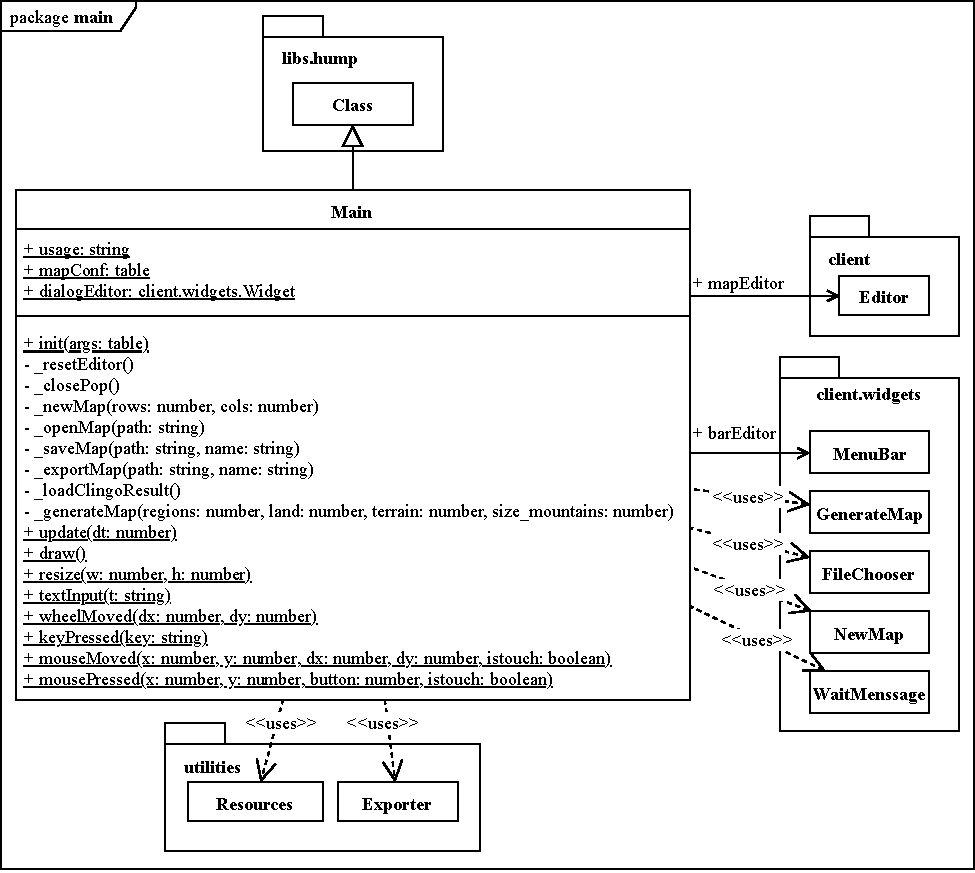
\includegraphics[width=\textwidth]{images/clase-principal.pdf}
	\caption{Diagrama de clases del paquete principal}
	\label{fig:mainclass}
\end{figure}

\subsubsection{Editor gráfico}
\label{subsubsec:client}

La clase \texttt{Editor} sirve como un subcontrolador para responder a las modificaciones y cambios de representación del mapa, ya sea cuando se actualiza este mediante uno de los casos de uso que recoge la clase principal [ver Sección \ref{subsubsec:main}] o cuando el usuario procede a la modificación del mapa, tal y como se explica en la Sección \ref{subsec:cases}. \\

Para ello, siguiendo el patrón decorador, esta se apoya en la clase \texttt{MapDecorator}, la cual se encarga de actualizar la vista del mapa, que es representada mediante una rejilla con los distintos terrenos mediante el objeto \texttt{love.SpriteBatch}, el cual es un mapa de \textit{tiles} bidimensional. Debido a que hay terrenos que contienen diferentes imágenes para las posiciones de un \textit{tile}, \texttt{MapDecorator} contiene varios métodos que permiten discretizarlas conociendo los vecinos de una celda. Finalmente esta clase llama al modelo en si, representado por la clase \texttt{Map}, la cual tiene una representación del mapa en forma de tabla. \\

Finalmente todas estas clases usan constantes que están definidas el módulo \texttt{Constants}.

\begin{figure}
	\centering
	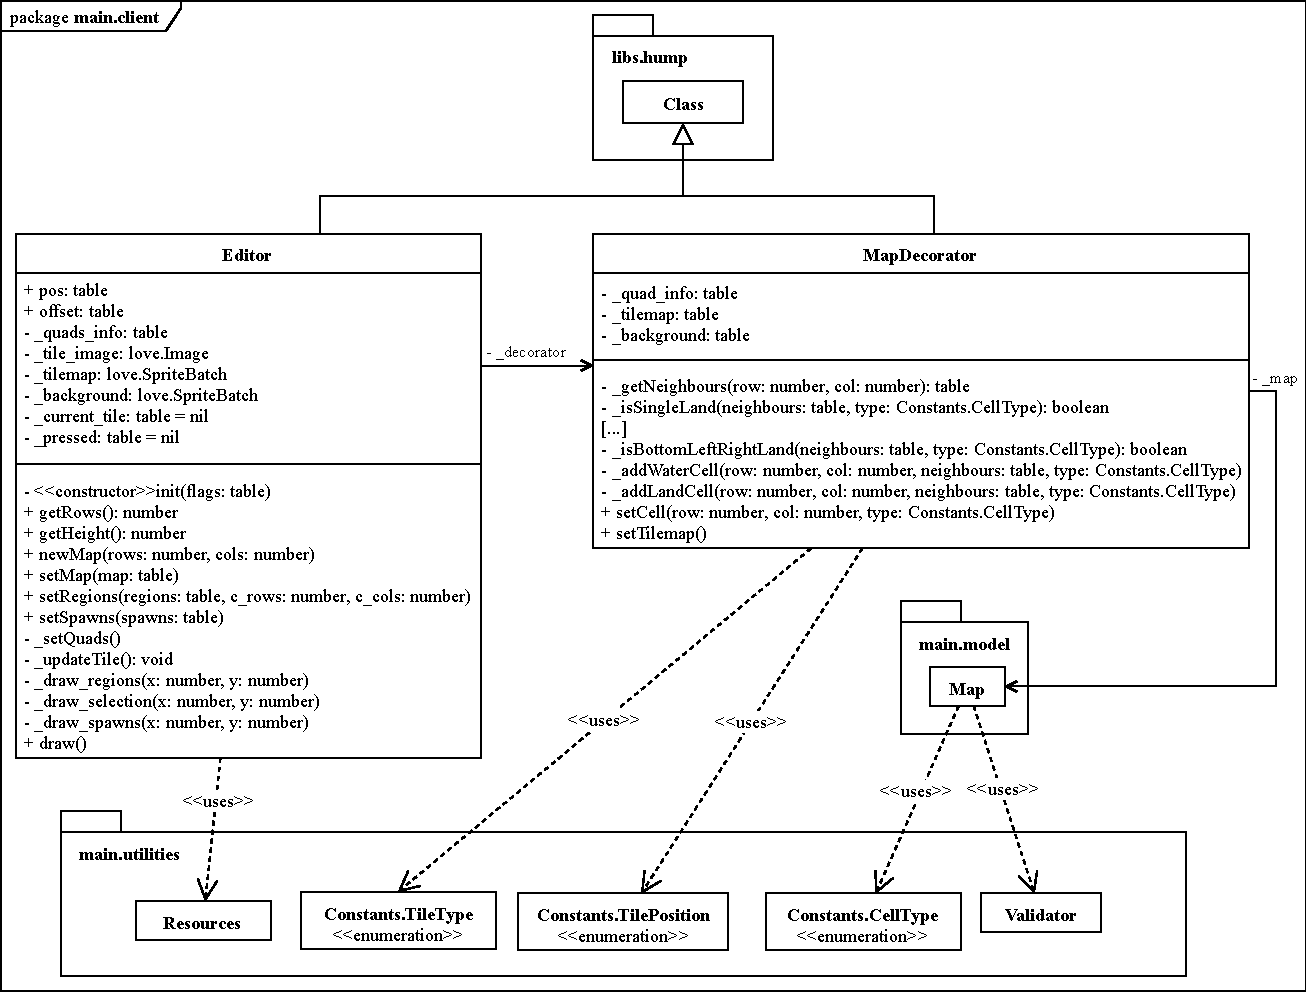
\includegraphics[width=\textwidth]{images/clase-editor.pdf}
	\caption{Diagrama de clases del paquete \texttt{Client}}
	\label{fig:editorclass}
\end{figure}

\subsubsection{Elemento gráficos complejos}
\label{subsubsec:widgets}

\begin{figure}
	\centering
	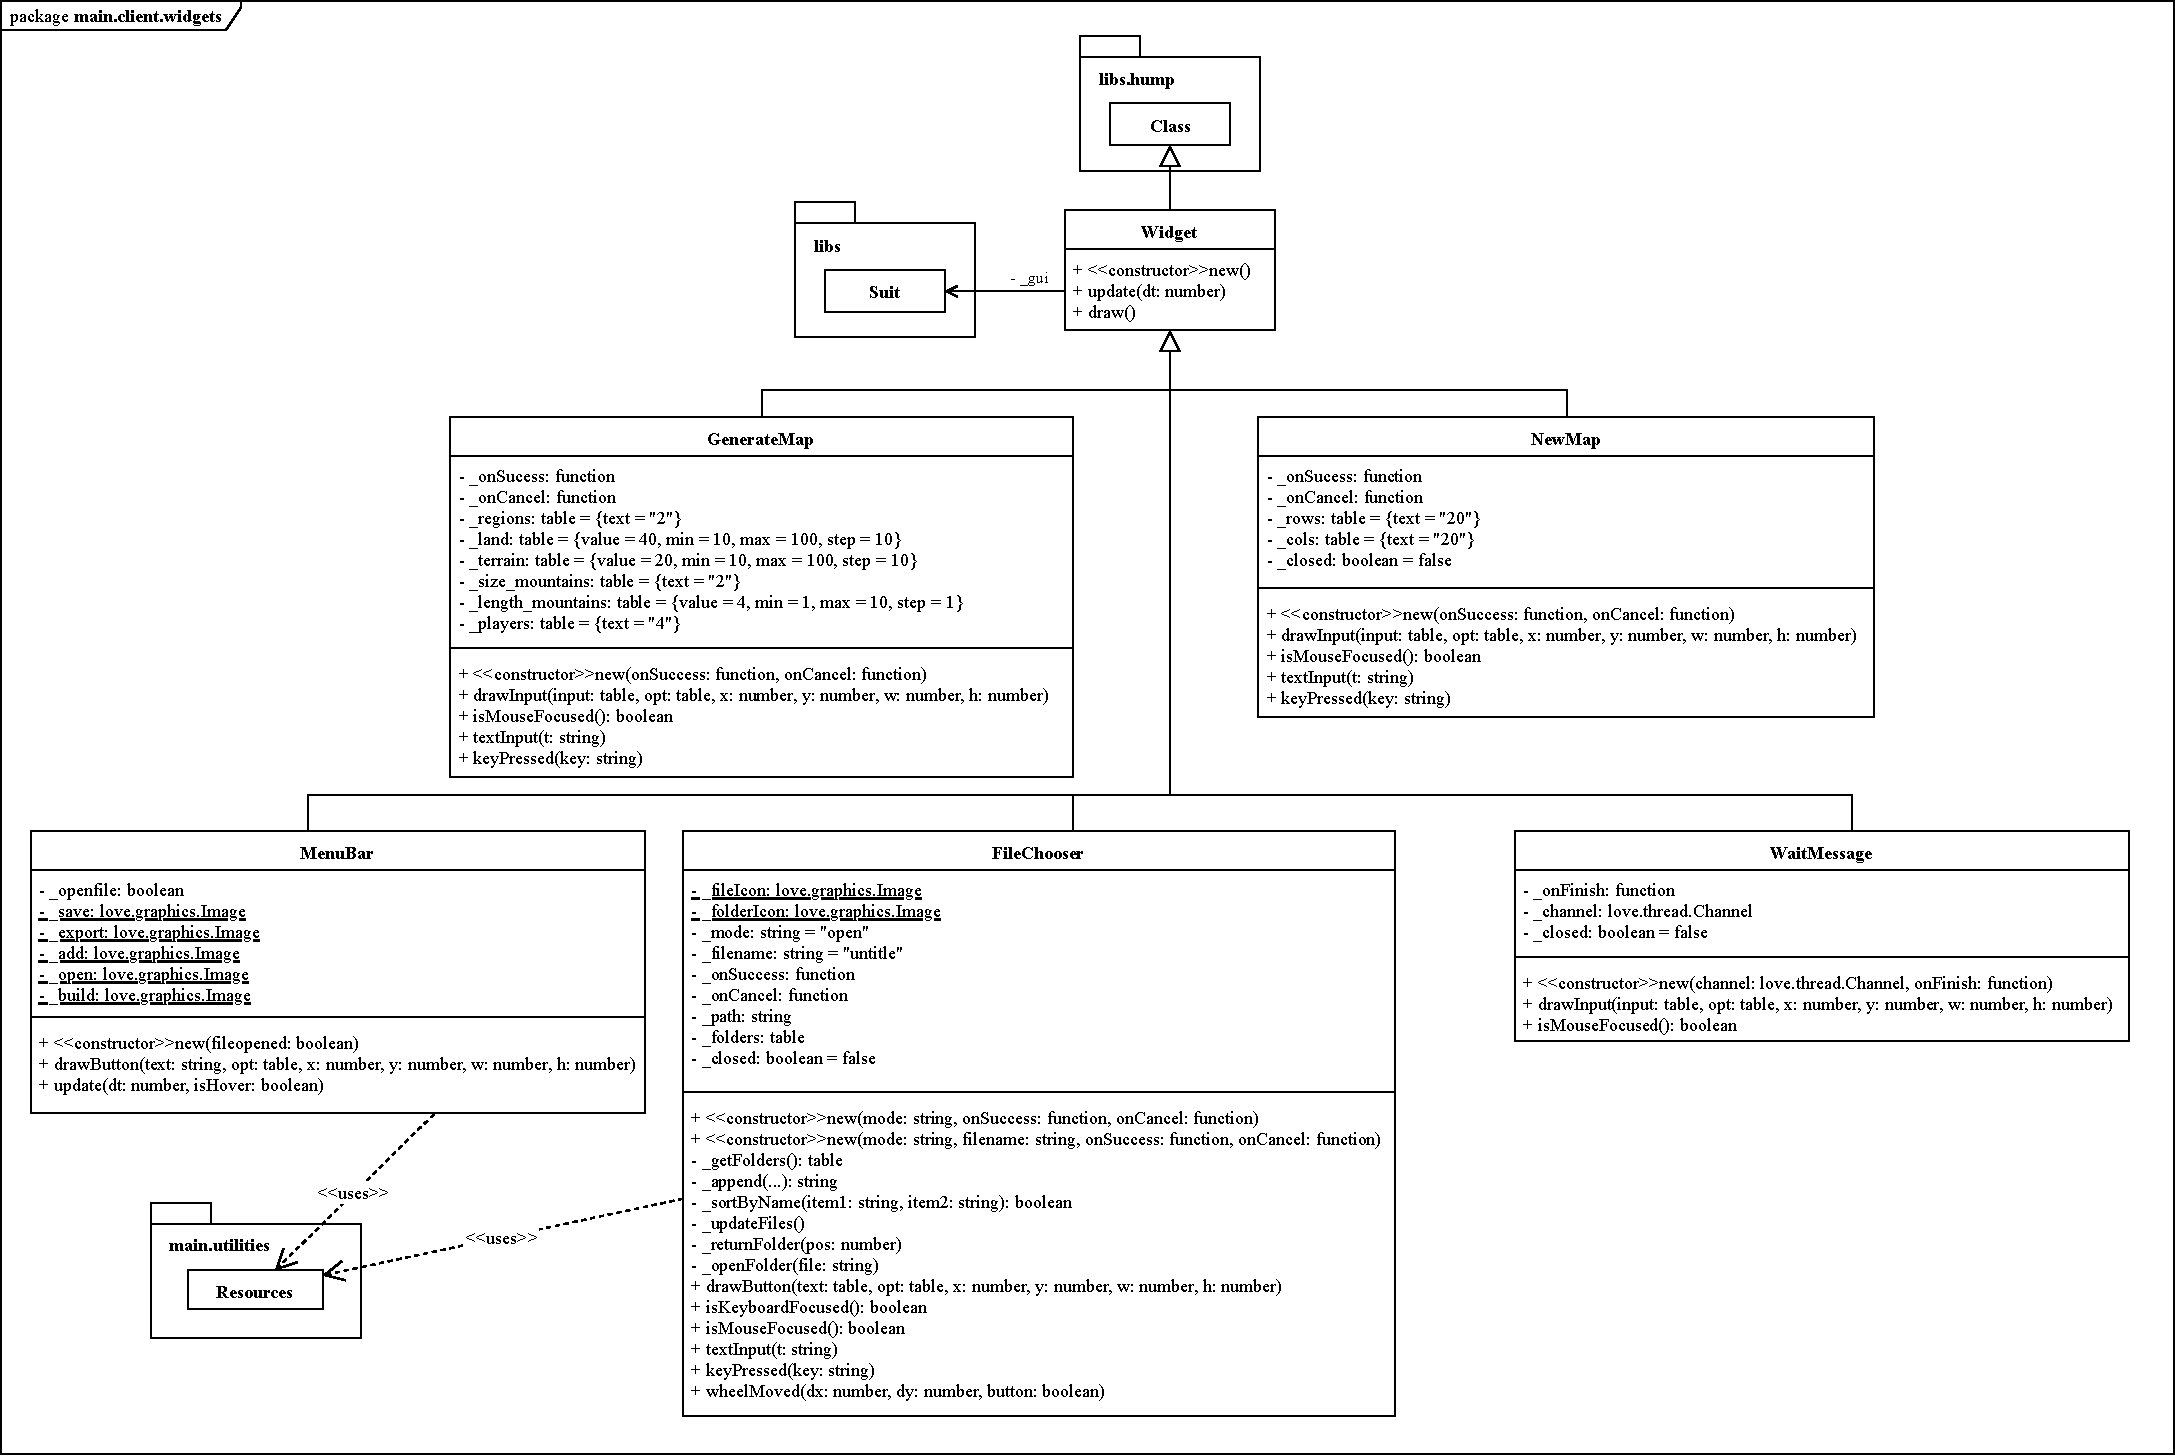
\includegraphics[width=\textwidth]{images/clases-widgets.pdf}
	\caption{Diagrama de clases del paquete \texttt{Widget}}
	\label{fig:widgetclasses}
\end{figure}

\subsubsection{Generador de mapas}
\label{subsubsec:generator}

\begin{figure}
	\centering
	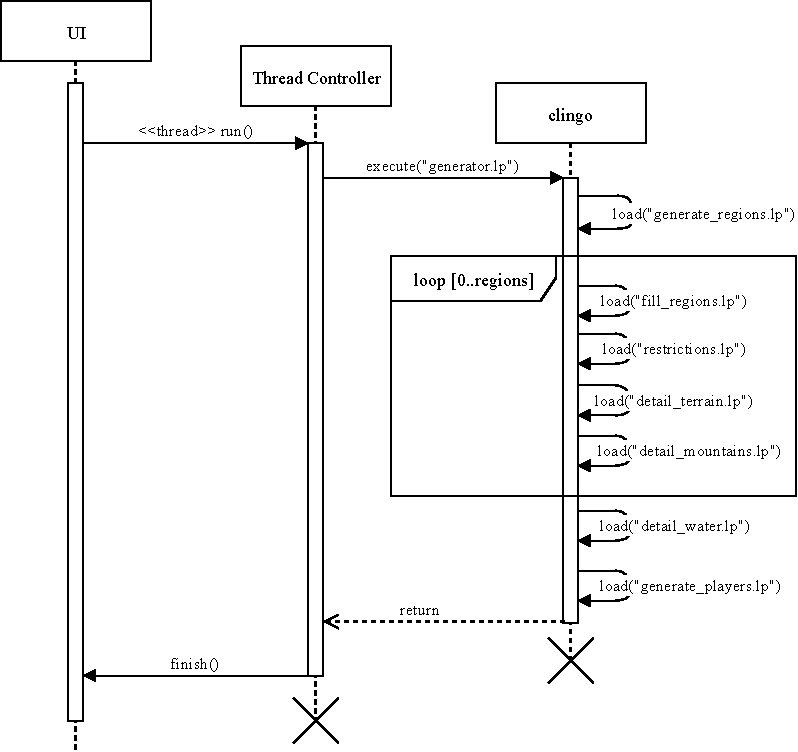
\includegraphics[width=\textwidth]{images/secuencia.pdf}
	\caption{Diagrama de secuencia de la ejecución del generador}
	\label{fig:sequence}
\end{figure}